\documentclass[11pt,a4paper]{amsart}
\usepackage[utf8]{inputenc}
\usepackage[T1]{fontenc}
\usepackage{lmodern}
\usepackage{amsmath,amssymb,amsthm}
\usepackage{booktabs}
\usepackage{graphicx}
\usepackage[margin=2.4cm]{geometry}
\usepackage{xcolor}
\usepackage[colorlinks=true,linkcolor=blue!50!black,citecolor=blue!50!black,urlcolor=blue!50!black]{hyperref}

\newtheorem{theorem}{Theorem}[section]
\newtheorem{lemma}[theorem]{Lemma}
\newtheorem{proposition}[theorem]{Proposition}
\newtheorem{corollary}[theorem]{Corollary}
\newtheorem*{theoremA}{Theorem A}
\newtheorem*{theoremB}{Theorem B}
\theoremstyle{remark}
\newtheorem{remark}[theorem]{Remark}
\newtheorem{example}[theorem]{Example}

\newcommand{\F}{\mathbb{F}}
\newcommand{\Fq}{\mathbb{F}_q}
\newcommand{\Tr}{\mathrm{Tr}}
\newcommand{\I}{\mathbb{I}}
\newcommand{\fC}{\mathfrak{C}}
\newcommand{\ord}{\mathrm{ord}}
\newcommand{\mat}[4]{\bigl(\begin{smallmatrix}#1&#2\\#3&#4\end{smallmatrix}\bigr)}

\title[Coefficients of invariant irreducible polynomials]{Prescribing coefficients of invariant irreducible
polynomials over finite fields: counterexamples, corrected formulas, and complete restoration}
\author{Ruqing Chen}
\address{GUT Geoservice Inc., Montreal, Canada}
\email{ruqing@hotmail.com}
\date{November 17, 2026}
\subjclass[2020]{11T06, 11T23, 11T55}
\keywords{irreducible polynomials, prescribed coefficients, invariant polynomials, finite fields, character sums}

\begin{document}
\begin{abstract}
For a lower-triangular $A\in\mathrm{GL}(2,q)$, G.~Kapetanakis (J.~Number Theory 180 (2017)) studied which
coefficients of the monic irreducible polynomials over $\Fq$ invariant under $A$ are forced and which can be
prescribed. We show that several statements of that paper are false or unproved: the coefficient formula of its
Theorem~2.8 is wrong; its inequality~(5) cannot hold for $\mu=2$ when $q\le64$, so that every row of its
Table~2 fails; Theorem~3.4(2) is false, the coefficient taking a single value instead of $\varphi(r)(q-1)/r$
values; the diagonal case of Theorem~3.4 is misstated twice; and the proof of Theorem~3.4(3) does not control
the constant term. We then give complete statements and proofs. Counting directly over all admissible residue
classes modulo $X^{\mu+1}$, without the von Mangoldt weights of the original argument, we prove both existence
statements with no exceptional pairs at all: for one eigenvalue, every $\kappa\in\Fq$ occurs whenever
$2\le\mu\le n/2$; for two eigenvalues, whenever $1\le\mu<n/2$. The finitely many cases not reached by the bounds
are settled by explicit polynomials.
\end{abstract}
\maketitle

\section{Introduction}

\subsection{The problem}
Let $q$ be a power of a prime $p$. For $A=\mat abcd\in\mathrm{GL}(2,q)$ and $F\in\Fq[X]$ put
$A\circ F=(bX+d)^{\deg F}F\bigl(\tfrac{aX+c}{bX+d}\bigr)$. Let $\I_n$ be the set of monic irreducible polynomials
of degree $n$ over $\Fq$, $\pi_q(n)=|\I_n|$, and let $\I_n^A$ be the set of $Q\in\I_n$ with $A\circ Q=\lambda Q$
for some $\lambda\in\Fq^*$. Coefficients are written $F=\sum f_iX^i$, and $\Tr$ is the trace $\Fq\to\F_p$. We
take $A=\mat a0cd$ lower-triangular, so that $A\circ F=d^{\deg F}F\bigl(\tfrac{aX+c}{d}\bigr)$; there are two cases.

\emph{One eigenvalue} ($a=d$). Then $A\circ F\sim F(X+\alpha)$ with $\alpha=c/d$; we assume $\alpha\ne0$.

\emph{Two eigenvalues} ($a\ne d$). Then $A\circ F\sim F(\rho X+c/d)$ with $\rho=a/d\ne1$. We write $r>1$ for the
order of $\rho$ in $\Fq^*$, $x_0=c/(d-a)$ for the fixed point of $X\mapsto\rho X+c/d$, and
\[
\fC=\{x\in\Fq^*:\gcd(r,(q-1)/\ord(x))=1\},\qquad|\fC|=\varphi(r)(q-1)/r .
\]
The question of \cite{K} is: given $0\le m\le n'$, which values does the coefficient $q_m$ take as $Q$ runs
through $\I^A_{n'}$? The answers there are its Theorem~2.8 (one eigenvalue) and Theorem~3.4 (two eigenvalues).

\subsection{Results}
For one eigenvalue write $n'=pn$ and, for $0\le m\le pn$ and $0\le i\le n$,
\begin{equation}\label{eq:gamma}
\gamma_i=\binom{n-i}{k}\bigl(-\alpha^{p-1}\bigr)^{n-i-k},\qquad k=\frac{m-n+i}{p-1},
\end{equation}
if $\max(0,n-m)\le i\le n-\lceil m/p\rceil$ and $i\equiv n-m\pmod{p-1}$, and $\gamma_i=0$ otherwise. Let $\mu$ be
the largest $i$ with $\gamma_i\ne0$, if there is one.

\begin{theoremA}
Let $A=\mat10\alpha1$ with $\alpha\in\Fq^*$.
\begin{enumerate}
\item[(0)] $\I^A_{n'}\ne\emptyset$ if and only if $p\mid n'$, and
$\I^A_{pn}=\{P(X^p-\alpha^{p-1}X):P\in\I_n,\ \Tr(p_{n-1}/\alpha^p)\ne0\}$.
\item[(1)] For $Q=P(X^p-\alpha^{p-1}X)$ and every $m$ we have $q_m=\sum_{i}\gamma_i\,p_{n-i}$. If no $\mu$ exists,
$q_m=0$ for all $Q\in\I^A_{pn}$.
\item[(2)] If $\mu=0$, then $q_m=\gamma_0$ for all $Q\in\I^A_{pn}$.
\item[(3)] If $\mu=1$, the values of $q_m$ on $\I^A_{pn}$ are exactly the $\gamma_0+\gamma_1\kappa$ with
$\Tr(\kappa/\alpha^p)\ne0$.
\item[(4)] If $2\le\mu\le n/2$, every $\kappa\in\Fq$ is a value of $q_m$ on $\I^A_{pn}$.
\item[(5)] The conclusion of (4) also holds for $2\le\mu\le n-1$ if $q^{(n-\mu-1)/2}\ge1.5\mu+5$.
\end{enumerate}
\end{theoremA}

For two eigenvalues write $n'=rn$ and, for $0\le m\le rn$ and $0\le i\le n-\lceil m/r\rceil$,
\begin{equation}\label{eq:delta}
\delta_i=\binom{(n-i)r}{m}(-x_0)^{(n-i)r-m}\qquad(0^0=1),
\end{equation}
and let $\mu$ be the largest $i$ with $\delta_i\ne0$, if there is one. Let $W(r)$ be the number of square-free
divisors of $r$.

\begin{theoremB}
Let $A=\mat a0cd$ with $a\ne d$, and $\rho$, $r$, $x_0$, $\fC$ as above.
\begin{enumerate}
\item[(0)] $\I^A_1=\{X-x_0\}$. For $n'>1$, $\I^A_{n'}\ne\emptyset$ if and only if $r\mid n'$, and
$\I^A_{rn}=\{P((X-x_0)^r):P\in\I_n,\ (-1)^np_0\in\fC\}$. For such $Q$ and every $m$,
$q_m=\sum_i\delta_i\,p_{n-i}$.
\item[(1)] Let $x_0=0$. Then $q_m=0$ unless $r\mid m$, and $q_{jr}=p_j$. The constant terms $q_0$ are exactly
the $x$ with $(-1)^nx\in\fC$. If $n\ge2$, $0<m<n'$ and $r\mid m$, every $\kappa\in\Fq$ is a value of $q_m$, except
that $\kappa=0$ is not a value when $n=2$ and either $q$ is even, or $q\equiv3\pmod4$ and $r$ is even.
\item[(2)] Let $x_0\ne0$. If no $\mu$ exists, $q_m=0$ on $\I^A_{rn}$. If $\mu=0$, then $q_m=\delta_0$ on
$\I^A_{rn}$; in particular $q_m=\binom{n'}{m}(-x_0)^{n'-m}$ for $n'-r<m<n'$.
\item[(3)] Let $x_0\ne0$. If $1\le\mu<n/2$, every $\kappa\in\Fq$ is a value of $q_m$ on $\I^A_{rn}$.
\item[(4)] The conclusion of (3) also holds for $1\le\mu\le n-1$ if $q^{(n-\mu-1)/2}\ge W(r)(\mu+3)$.
\end{enumerate}
\end{theoremB}

Items A(4) and B(3) have no exceptions. In \cite{K} they are asserted for ``$q\ge65$ or $n\ge26$''
(Theorem~2.8(4)) and for ``$n\ge5$ and $q\ge31$, or $n\ge47$'' (Theorem~3.4(3)), with intermediate ranges
in Tables~2 and~3; we show in Section~\ref{sec:K} that those ranges are not established there. The other
differences from \cite{K} are: the formula \eqref{eq:gamma}; item B(2), where \cite{K} claims $|\fC|$ values;
and item B(1), where \cite{K} has the condition $q_0\in\fC$ and no exception.

\subsection{Source}
We checked \cite{K} in the author's repository text dated 24~May 2017 (``Preprint submitted to Journal of
Number Theory''). Theorem, equation and table numbers of \cite{K} are those of that text; the printed version
was not compared and may differ. On 17~November 2026 Crossref listed no corrigendum, erratum or update for
\cite{K}.

\section{Tools}\label{sec:tools}

\subsection{Counting irreducibles in residue classes}
Let $R_n=q^n-n\pi_q(n)=\sum_{k\mid n,\,k<n}k\,\pi_q(k)$. Since $k\pi_q(k)\le q^k$ and the proper divisors of
$n$ are $n/2$ and numbers $\le n/3$, one checks that
\begin{equation}\label{eq:Rn}
R_n\le2q^{n/2},\qquad\text{hence}\qquad n\,\pi_q(n)\ge q^n-2q^{n/2}.
\end{equation}
A \emph{Dirichlet character modulo} $X^D$ is a character $\chi$ of $(\Fq[X]/X^D)^*$, extended by $\chi(F)=0$ if
$X\mid F$.

\begin{lemma}\label{lem:weil}
Let $\chi$ be a non-trivial Dirichlet character modulo $X^D$, $D\ge1$. Then
\[
\Bigl|\sum_{T\in\I_n}\chi(T)\Bigr|\le B_n(D):=\frac{(D-1)q^{n/2}+R_n}{n}.
\]
If $\chi$ is trivial on $\Fq^*$, the sum is also at most $(Dq^{n/2}+1)/n$; we write $B^e_n(D)$ for the smaller of
the two bounds.
\end{lemma}
\begin{proof}
Let $c_n(\chi)=\sum_{d\mid n}\frac nd\sum_{T\in\I_{n/d}}\chi(T)^d$. Weil's theorem gives
$|c_n(\chi)|\le(D-1)q^{n/2}$ \cite[Theorem~2.5]{K}, \cite[Ch.~4]{Ro}. The terms with $d>1$ have total modulus at
most $R_n$, which gives the first bound. The second is \cite[Proposition~2.6]{K}, from \cite[Corollary~2.8]{Wa}.
\end{proof}

Fix $\mu\ge1$ and let $U=(\Fq[X]/X^{\mu+1})^*$, of order $(q-1)q^\mu$. Then $U=\Fq^*\times U^1$, where $U^1$ is
the group of classes $g$ with $g(0)=1$, of order $q^\mu$; a class is determined by $g_1,\dots,g_\mu$. A
character $\lambda$ of $U^1$ has \emph{level} $j$ if $j$ is least such that $\lambda$ factors through
$g\bmod X^{j+1}$; there are $q^\mu-q^{\mu-1}$ characters of level $\mu$. Every character of $U$ is
$\eta\otimes\lambda$ with $\eta$ a character of $\Fq^*$, and as a Dirichlet character it sends $T$ to
$\eta(T(0))\lambda(T/T(0))$. For a subset $S$ of a finite abelian group $G$ write
$\widehat S(\lambda)=\sum_{s\in S}\overline{\lambda(s)}$; then $\sum_\lambda|\widehat S(\lambda)|^2=|G|\,|S|$.

\subsection{Two existence lemmas}

\begin{lemma}\label{lem:trace}
For every $n\ge1$ and $t\in\Fq^*$ there is $P\in\I_n$ with $p_{n-1}=t$.
\end{lemma}
\begin{proof}
There are $q^{n-1}$ elements $\beta\in\F_{q^n}$ with $\Tr_{q^n/q}(\beta)=-t$. Those of degree less than $n$ lie
in some $\F_{q^{n/\ell}}$, $\ell$ a prime divisor of $n$, where the trace is $\ell$ times the trace to $\Fq$; so
there are at most $\sum_\ell q^{n/\ell-1}<q^{n-1}$ of them. Take the minimal polynomial of one of the others.
\end{proof}

\begin{lemma}\label{lem:norm}
For every $n\ge2$ and $x\in\Fq^*$ there is $P\in\I_n$ with $p_0=x$.
\end{lemma}
\begin{proof}
There are $(q^n-1)/(q-1)$ elements of $\F_{q^n}$ of norm $(-1)^nx$. In $\F_{q^{n/\ell}}$ the norm to $\Fq$ is
the $\ell$-th power of the norm from $\F_{q^{n/\ell}}$, so at most $\ell(q^{n/\ell}-1)/(q-1)$ of them lie there,
and $\sum_\ell\ell(q^{n/\ell}-1)<q^n-1$ for $n\ge2$.
\end{proof}

\section{One eigenvalue}\label{sec:one}

\begin{proposition}\label{prop:periodic}
Let $\alpha\in\Fq^*$ and $Y=X^p-\alpha^{p-1}X$. A polynomial $F\in\Fq[X]$ satisfies $F(X+\alpha)=F(X)$ if and only
if $F=G(Y)$ for some $G\in\Fq[X]$.
\end{proposition}
\begin{proof}
$Y=\prod_{j\in\F_p}(X-j\alpha)$ is invariant, so every $G(Y)$ is. Conversely let $F$ be invariant and write
$F=G_1Y+H$ with $\deg H<p$. Then $G_1(X+\alpha)Y+H(X+\alpha)=G_1Y+H$, so $Y$ divides $H(X+\alpha)-H(X)$, which
has degree $<p$ and is therefore $0$. Then $H-H(0)$ has the $p$ roots $j\alpha$ and degree $<p$, so $H=f_0$,
and $G_1$ is again invariant. Induction on the degree gives $F=G(Y)$.
\end{proof}

By Agou's theorem \cite{Ag}, \cite[Theorem~2.2]{K}, for $P\in\I_n$ the polynomial $P(X^p-\alpha^{p-1}X)$ is
irreducible if and only if $\Tr(p_{n-1}/\alpha^p)\ne0$. Since $A\circ F\sim F(X+\alpha)$ and both are monic up to
the scalar, $Q\in\I^A_{n'}$ means $Q(X+\alpha)=Q(X)$; by Proposition~\ref{prop:periodic}, $Q=G(Y)$ with $G$
irreducible. This proves A(0), non-emptiness being Lemma~\ref{lem:trace}.

\begin{proof}[Proof of A(1)--(3)]
We have $Q=\sum_j p_j\sum_k\binom jk(-\alpha^{p-1})^{j-k}X^{pk+j-k}$. The exponent equals $m$ for
$k=(m-j)/(p-1)$, which requires $j\equiv m\pmod{p-1}$ and $0\le k\le j$, that is, $\lceil m/p\rceil\le j\le
\min(m,n)$. Putting $j=n-i$ gives $q_m=\sum_i\gamma_ip_{n-i}$ with $\gamma_i$ as in \eqref{eq:gamma}. Items (1)
and (2) follow, since $p_n=1$. For (3), $q_m=\gamma_0+\gamma_1p_{n-1}$, and by Lemma~\ref{lem:trace} every
$\kappa$ with $\Tr(\kappa/\alpha^p)\ne0$ is $p_{n-1}$ for some $P\in\I_n$.
\end{proof}

Items (4) and (5) rest on the following count.

\begin{proposition}\label{prop:D2}
Let $n\ge3$, $2\le\mu\le n-1$, $c\in\Fq^*$, $\gamma_0,\dots,\gamma_\mu\in\Fq$ with $\gamma_\mu\ne0$, and
$\kappa\in\Fq$. The number $N$ of $P\in\I_n$ with $\Tr(c\,p_{n-1})\ne0$ and $\sum_{i=0}^\mu\gamma_ip_{n-i}=\kappa$
satisfies
\begin{equation}\label{eq:D2}\tag{D2}
N\ \ge\ \frac{p-1}{pq}\bigl(\pi_q(n)-B^e_n(2)\bigr)-\Bigl(1-\frac1q\Bigr)\sqrt{\frac{(p-1)q^{\mu-1}}{p}}\;B^e_n(\mu+1).
\end{equation}
\end{proposition}
\begin{proof}
For $P\in\I_n$ let $g=X^nP(1/X)$, so $g_i=p_{n-i}$ and $g(0)=1$, and $T=g/p_0\in\I_n$; then $P\mapsto T$ is a
bijection of $\I_n$, and $\lambda(T)=\lambda(g)$ for every character $\lambda$ of $U^1$ (extended trivially on
$\Fq^*$). Let $S\subset U^1$ be the set of classes with $\Tr(c\,g_1)\ne0$ and
$\gamma_0+\sum_{i\ge1}\gamma_ig_i=\kappa$. Here $g_1$ takes $q(p-1)/p$ values, $g_2,\dots,g_{\mu-1}$ are free and
$g_\mu$ is determined, so $|S|=(p-1)q^{\mu-1}/p$. By orthogonality,
\[
N=\frac1{q^\mu}\sum_\lambda\widehat S(\lambda)\sum_{T\in\I_n}\lambda(T).
\]
Let $\psi(g)=e^{2\pi i\Tr(c\,g_1)/p}$, a character of $U^1$ of level $1$ and order $p$. If $\lambda$ has level
less than $\mu$, it only sees $g_1,\dots,g_{\mu-1}$, on which $S$ projects bijectively onto the complement of
$\ker\psi$; hence $\widehat S(\lambda)=-|\ker\psi|=-|S|/(p-1)$ if $\lambda\in\langle\psi\rangle$, $\lambda\ne1$,
and $\widehat S(\lambda)=0$ for all other non-trivial $\lambda$ of level $<\mu$. By the Parseval identity the
characters of level $\mu$ therefore satisfy
\[
\sum_{\mathrm{level}\ \mu}|\widehat S(\lambda)|^2=q^\mu|S|-|S|^2-\frac{|S|^2}{p-1}=|S|\,(q^\mu-q^{\mu-1}),
\]
and by Cauchy--Schwarz $\sum_{\mathrm{level}\ \mu}|\widehat S(\lambda)|\le(q^\mu-q^{\mu-1})\sqrt{|S|}$. The
characters $\psi^j$ are characters modulo $X^2$ and those of level $\mu$ are characters modulo $X^{\mu+1}$, all
trivial on $\Fq^*$. Lemma~\ref{lem:weil} gives
$q^\mu N\ge|S|\pi_q(n)-|S|B^e_n(2)-(q^\mu-q^{\mu-1})\sqrt{|S|}\,B^e_n(\mu+1)$.
\end{proof}

\begin{lemma}\label{lem:D2pos}
The right-hand side of \eqref{eq:D2} is positive if $q^{(n-\mu-1)/2}\ge1.5\mu+5$. For $2\le\mu\le n/2$ it is
positive except for the $15$ triples
\[
\begin{aligned}
(q,n,\mu)={}&(2,4,2),(2,5,2),(2,6,2),(2,6,3),(2,8,4),(2,10,5),(3,4,2),(3,6,3),\\
&(4,4,2),(4,6,3),(5,4,2),(7,4,2),(8,4,2),(9,4,2),(16,4,2).
\end{aligned}
\]
\end{lemma}
\begin{proof}
Positivity means $\pi_q(n)-B^e_n(2)>(q-1)\sqrt{pq^{\mu-1}/(p-1)}\,B^e_n(\mu+1)$. By \eqref{eq:Rn},
$B^e_n(D)\le(Dq^{n/2}+1)/n$ and $p/(p-1)\le2$ it suffices that
$q^n-4q^{n/2}-1>\sqrt2\,q^{(\mu+1)/2}\bigl((\mu+1)q^{n/2}+1\bigr)$. Dividing by $q^{(n+\mu+1)/2}$ and using
$q^{(\mu+1)/2}\ge2^{3/2}$, this holds if $q^{(n-\mu-1)/2}\ge1.42\mu+3.5$. If $\mu\le n/2$ the exponent is at
least $n/4-1/2$ and $1.5\mu+5\le0.75n+5$, so the condition holds when $q^{n/4-1/2}\ge0.75n+5$, that is, for
$q\ge64$ and all $n\ge4$, and for $n>60$ and all $q$. In the remaining range $q<64$, $4\le n\le60$ we evaluated
the right-hand side of \eqref{eq:D2}; it is positive except in the listed cases.
\end{proof}

\begin{proof}[Proof of A(4) and A(5)]
Apply Proposition~\ref{prop:D2} with $c=\alpha^{-p}$ and the $\gamma_i$ of \eqref{eq:gamma}: every $P$ counted
gives $Q=P(X^p-\alpha^{p-1}X)\in\I^A_{pn}$ with $q_m=\kappa$. By Lemma~\ref{lem:D2pos}, $N>0$ under the
hypothesis of (5), and under that of (4) outside the $15$ listed triples. For those triples we searched, for
every $c\in\Fq^*$, every $(\gamma_1,\dots,\gamma_{\mu-1})\in\Fq^{\mu-1}$ with $\gamma_\mu=1$, $\gamma_0=0$, and every
$\kappa$, for a polynomial $P$ as in Proposition~\ref{prop:D2}: one exists in each of the $5710$ cases
(Table~\ref{tab:wit}).
\end{proof}

\section{Two eigenvalues}\label{sec:two}

\begin{proposition}\label{prop:struct}
Let $A=\mat a0cd$ with $a\ne d$. A monic polynomial $Q$ satisfies $A\circ Q\sim Q$ if and only if
$Q=(X-x_0)^kG((X-x_0)^r)$ for some $k\ge0$ and $G\in\Fq[X]$.
\end{proposition}
\begin{proof}
$A\circ Q\sim Q(\rho X+c/d)$, and $\rho X+c/d-x_0=\rho(X-x_0)$. So with $R(Y)=Q(Y+x_0)$ the condition is
$R(\rho Y)\sim R(Y)$. If $R=\sum f_iY^i$ has lowest term $f_kY^k$ and highest $f_{k+s}Y^{k+s}$, comparing these
two coefficients gives $\rho^s=1$ and $R(\rho Y)=\rho^kR(Y)$, hence $f_i=0$ unless $r\mid i-k$. The converse is
clear.
\end{proof}

For irreducible $Q$ of degree $n'>1$ this gives $k=0$ and $Q=P((X-x_0)^r)$ with $P\in\I_n$. By Cohen's
criterion \cite{Co}, \cite[Theorem~3.2]{K}, since $r\mid q-1$, $P(X^r)$ is irreducible if and only if
$\gcd(r,(q-1)/e)=1$ for $e$ the order of $(-1)^np_0$, that is, $(-1)^np_0\in\fC$. Expanding
$(X-x_0)^{jr}$ gives $q_m=\sum_j\binom{jr}{m}(-x_0)^{jr-m}p_j$, the sum over $\lceil m/r\rceil\le j\le n$; with
$j=n-i$ this is $\sum_i\delta_ip_{n-i}$. This proves B(0); non-emptiness follows from Lemma~\ref{lem:norm}. Item
B(2) is immediate, since $p_n=1$.

\begin{proof}[Proof of B(1)]
For $x_0=0$, $Q=P(X^r)$, so $q_{jr}=p_j$ and the other coefficients vanish. The constant terms are the $p_0$
with $(-1)^np_0\in\fC$, all of which occur by Lemma~\ref{lem:norm} (for $n=1$ take $P=X+p_0$). Now let $n\ge2$ and
$0<j<n$. By the Hansen--Mullen primitivity theorem \cite{Co2,CP1,CP2}, \cite[Theorem~1.2]{K}, there is a
primitive $P\in\I_n$ with $p_j=\kappa$, unless $n=2$ and $\kappa=0$, or $(q,n)=(4,3)$ and $\kappa=0$ (the third
exception there has $q=2$, where no $r>1$ exists). A primitive $P$ has $(-1)^np_0$ primitive, hence in $\fC$.
For $(q,n)=(4,3)$, $r=3$, take $P=X^3+\omega$ with $\omega$ of order $3$. For $n=2$, $\kappa=0$ we need
$X^2+p_0$ irreducible with $p_0\in\fC$. If $q$ is even, $X^2+p_0$ is a square. Let $q$ be odd; then $-p_0$ must
be a non-square. An element $x$ lies in $\fC$ if and only if $\ord(x)$ contains the full $\ell$-part of $q-1$
for every prime $\ell\mid r$. If $r$ is even, $p_0\in\fC$ is a non-square, so $-1$ is a square and
$q\equiv1\pmod4$; then any primitive $p_0$ works. If $r$ is odd, take $p_0=-g$ with $g$ primitive: $-p_0=g$
is a non-square, and $\ord(-g)$ is $q-1$ or $(q-1)/2$, so it contains the full $\ell$-part of $q-1$ for every
odd $\ell$.
\end{proof}

\begin{proposition}\label{prop:D3}
Let $n\ge2$, $1\le\mu\le n-1$, $\delta_1,\dots,\delta_\mu\in\Fq$ with $\delta_\mu\ne0$ and $\kappa\in\Fq$. The
number $N$ of $P\in\I_n$ with $(-1)^np_0\in\fC$ and $\sum_{i=1}^\mu\delta_ip_{n-i}=\kappa$ satisfies
\begin{equation}\label{eq:D3}\tag{D3}
N\ \ge\ \frac{|\fC|}{q(q-1)}\Bigl(\pi_q(n)-(W(r)-1)B_n(1)-W(r)(q-1)q^{(\mu-1)/2}B_n(\mu+1)\Bigr).
\end{equation}
\end{proposition}
\begin{proof}
With $g=X^nP(1/X)$ and $T=g/p_0\in\I_n$ as before, $T(0)=p_0^{-1}$ and $T/T(0)=g$, so the class of $T$ in
$U=\Fq^*\times U^1$ is $(p_0^{-1},g)$. Let $\fC'=(-1)^n\fC$, let $H\subset U^1$ be the set of classes with
$\sum\delta_ig_i=\kappa$, of size $q^{\mu-1}$, and $S=\{(t,g):t^{-1}\in\fC',\ g\in H\}$. With
$s_\eta=\sum_{t^{-1}\in\fC'}\overline{\eta(t)}$,
\[
N=\frac1{(q-1)q^\mu}\sum_{\eta,\lambda}s_\eta\,\widehat H(\lambda)\sum_{T\in\I_n}\eta(T(0))\,\lambda(T/T(0)).
\]
The indicator of $\fC$ is $\sum_{d\mid\mathrm{rad}(r)}\frac{\mu(d)}d\sum_{\theta^d=1}\theta$, so $s_\eta=0$
unless the order $e$ of $\eta$ divides $\mathrm{rad}(r)$, and then $|s_\eta|=|\fC|/\varphi(e)$; summing over
$\eta$, $\sum_\eta|s_\eta|=|\fC|\,W(r)$. Since $\delta_\mu\ne0$, $H$ projects bijectively onto the classes modulo
$X^\mu$, so $\widehat H(\lambda)=0$ for non-trivial $\lambda$ of level $<\mu$, and by Parseval and
Cauchy--Schwarz
\[
\sum_{\mathrm{level}\ \mu}|\widehat H(\lambda)|\le\sqrt{(q^\mu-q^{\mu-1})(q^{2\mu-1}-q^{2\mu-2})}=(q-1)\,q^{\mu-1}q^{(\mu-1)/2}.
\]
The term $\eta=1$, $\lambda=1$ is $|\fC|q^{\mu-1}\pi_q(n)$. For $\lambda=1$, $\eta\ne1$ the character is one
modulo $X$, bounded by $B_n(1)$; for $\lambda$ of level $\mu$ it is one modulo $X^{\mu+1}$, bounded by
$B_n(\mu+1)$ (Lemma~\ref{lem:weil}). Collecting terms gives \eqref{eq:D3}.
\end{proof}

\begin{lemma}\label{lem:D3pos}
The right-hand side of \eqref{eq:D3} is positive if $q^{(n-\mu-1)/2}\ge W(r)(\mu+3)$. For $1\le\mu<n/2$ it is
positive except for $(q,r,n,\mu)=(3,2,4,1)$, $(7,6,4,1)$, $(7,6,5,2)$ and, with $n=3$, $\mu=1$, for the $18$
pairs
\[
\begin{aligned}
(q,r)={}&(3,2),(4,3),(5,2),(5,4),(7,6),(11,10),(13,6),(13,12),(16,15),(19,6),(19,18),\\
&(31,30),(43,42),(61,30),(61,60),(67,66),(71,70),(211,210).
\end{aligned}
\]
\end{lemma}
\begin{proof}
By \eqref{eq:Rn}, positivity follows from $q^{n/2}>2W+W(\mu+2)q^{(\mu+1)/2}$ with $W=W(r)$, hence from
$q^{(n-\mu-1)/2}\ge W(\mu+3)$, as $q^{(\mu+1)/2}\ge3$. Now $W(r)\le W(q-1)\le4.9\,q^{1/4}$, because
$W(t)/t^{1/4}\le\prod_{\ell<16}2\ell^{-1/4}<4.9$. For $\mu<n/2$ we have $\mu\le(n-1)/2$, so the condition holds
if $q^{(n-2)/4}\ge2.45(n+5)$: for $n\ge4$ this is true when $q\ge487$ or $n>60$, and for $n=3$ the condition
$q^{1/2}\ge4W(q-1)$ is true when $q\ge147579$. In the remaining ranges we evaluated the right-hand side of
\eqref{eq:D3} for every $r$; it is positive except in the listed cases.
\end{proof}

\begin{proof}[Proof of B(3) and B(4)]
Apply Proposition~\ref{prop:D3} with the $\delta_i$ of \eqref{eq:delta} and $\kappa-\delta_0$ in place of
$\kappa$. By Lemma~\ref{lem:D3pos}, $N>0$ under the hypothesis of (4), and under that of (3) outside the listed
cases. For those we searched, for every $(\delta_1,\dots,\delta_{\mu-1})$ with $\delta_\mu=1$ and every $\kappa$,
for a polynomial $P$ as in Proposition~\ref{prop:D3}: one exists in each of the $719$ cases
(Table~\ref{tab:wit}).
\end{proof}

\begin{table}[t]
\centering\small
\begin{tabular}{llll}
\toprule
case & data & $\kappa$ & polynomial $P$\\
\midrule
A, $(q,n,\mu)=(2,4,2)$ & $c=1$, $\gamma_1=0$ & $0$ & $X^4+X^3+1$\\
A, $(2,6,3)$ & $c=1$, $\gamma_1=\gamma_2=0$ & $0$ & $X^6+X^5+1$\\
A, $(2,8,4)$ & $c=1$, $\gamma_1=\gamma_2=\gamma_3=0$ & $0$ & $X^8+X^7+X^3+X^2+1$\\
A, $(2,10,5)$ & $c=1$, $\gamma_1=\dots=\gamma_4=0$ & $0$ & $X^{10}+X^9+X^4+X^2+1$\\
A, $(3,6,3)$ & $c=1$, $\gamma_1=\gamma_2=0$ & $0$ & $X^6+X^5+X^2+X+1$\\
A, $(5,4,2)$ & $c=1$, $\gamma_1=0$ & $0$ & $X^4+X^3+4X+1$\\
B, $(q,r,n,\mu)=(3,2,4,1)$ & & $0$ & $X^4+X^2+2$\\
B, $(7,6,4,1)$ & & $0$ & $X^4+X^2+3$\\
B, $(7,6,5,2)$ & $\delta_1=0$ & $0$ & $X^5+3X^2+2$\\
B, $(7,6,3,1)$ & & $0$ & $X^3+2$\\
\bottomrule
\end{tabular}
\caption{Examples of the polynomials $P$ found in the cases where \eqref{eq:D2} or \eqref{eq:D3} is not
positive ($\gamma_\mu=1$, resp.\ $\delta_\mu=1$). The complete lists, $5710$ and $719$ cases, are in the
repository \cite{Repo}.}\label{tab:wit}
\end{table}

\section{The statements of \texorpdfstring{\cite{K}}{[K]}}\label{sec:K}

We now compare with \cite{K}. Its structural results (Lemmas~2.1, 3.1, 3.3 and the use of the theorems of Agou
and Cohen) are correct, and its Table~1 is correct (Table~\ref{tab:one}). The following points are not.

\subsection{The coefficient formula of Theorem~2.8}
Theorem~2.8 prints $\gamma_i=\binom{n-i}{k}(-\alpha)^{p-n+i}$ for $i\equiv m-n\pmod{p-1}$. Compared with
\eqref{eq:gamma}: the exponent of $\alpha$ should be $(p-1)(n-i-k)=p(n-i)-m$; the sign $(-1)^{n-i-k}$ is lost for
odd $p$, where $(-\alpha)^{(p-1)j}$ was written for $(-\alpha^{p-1})^{j}$; and the congruence is reversed, which
matters for $p\ge5$, where $k$ then need not be an integer. Already in Table~1 of \cite{K} ($q=3$, $\alpha=2$,
$n=2$) both invariant sextics have $q_4=1$; \eqref{eq:gamma} gives $\gamma_0=1$ and the printed formula gives
$2$. Over all $1307$ triples $(\alpha,n,m)$ tested for $q\le9$ the printed formula is wrong in $595$ and
undefined in $52$ (Figure~\ref{fig:one}(a)). In Proposition~2.3 the polynomial $F$ should have
$f_i=\gamma_{\mu-i}\gamma_\mu^{-1}$, not $\gamma_{i-1}\gamma_\mu^{-1}$.

\subsection{Inequality (5) and Table 2}
For $2\le\mu\le n/2$, \cite{K} counts with von Mangoldt weights: with $F$ as above and $\psi$ as in the proof of
Proposition~\ref{prop:D2},
\[
w=\sum_{H}\Lambda(H)\,\#\bigl\{g:\ \psi(g)\ne1,\ gF\equiv H\ (\mathrm{mod}\ X^{\mu+1})\bigr\},
\]
the sum over $H$ of degree $<\mu$ with $H(0)=1$, and $g$ as in Proposition~\ref{prop:D2}. Writing
$w=A_\psi+B_\psi+C_\psi$ for the contributions of $\lambda=1$, of $\lambda\in\langle\psi\rangle\setminus\{1\}$
and of the other characters, it derives the sufficient condition~(5), whose left-hand side is
$q^{n/2}\bigl(q^{(\mu-1)/2}-4\mu\bigr)+4\mu/(q-1)$ and whose right-hand side exceeds $8\mu^2q^\mu$. If
$q^{(\mu-1)/2}\le4\mu$ the left-hand side is at most $4\mu$, so (5) fails for every $n$. This happens for
$\mu=2$ and all $q\le64$, for $\mu\le3$ if $q\le11$, and for $\mu\le12,7,5,4$ if $q=2,3,4,5$. Hence the claims
that (5) holds for $n\ge26$ and all $q$, and for the pairs of Table~2, are false: each row of Table~2 has
$q\le27$ and includes $\mu=2$. The claim for $q\ge67$ fails as well, at $(n,\mu)=(4,2)$ for $q\le1597$, at
$(5,2)$ for $q\le113$ and at $(6,3)$ for $q\le83$. Three steps of the derivation are at fault.

\emph{(i)} Equation~(2) evaluates $\sum_H\Lambda(H)$ as $(q^\mu-1)/(q-1)$. The powers of $X$ and $H=1$ must be
left out: the sum is $L=\sum_{j=1}^{\mu-1}(q^j-1)$, e.g.\ $1$ instead of $3$ for $q=\mu=2$. \emph{(ii)} For
$\lambda\in\langle\psi\rangle$ the sum $\sum_H\Lambda(H)\bar\lambda(H)$ is bounded by
$\mu(q^{\mu/2}-1)/(q^{1/2}-1)$, which is what produces the term $4\mu$. \emph{(iii)} Proposition~2.6 gives
$(\deg M\cdot q^{n/2}+1)/n$ with $\deg M=\mu+1$, but $\mu q^{n/2}/n$ is used.

\begin{proposition}\label{prop:AB}
Let $N^*$ be the number of $P\in\I_n$ with $\Tr(p_{n-1}/\alpha^p)\ne0$. Then
\[
A_\psi+B_\psi=\frac{N^*}{q^\mu}\bigl(L+(\mu-1)\varepsilon\bigr),\qquad
\varepsilon=1\ \text{if }\psi(F)=1,\quad\varepsilon=-\tfrac1{p-1}\ \text{otherwise}.
\]
\end{proposition}
\begin{proof}
By orthogonality, $w=q^{-\mu}\sum_\lambda\lambda(F)\bigl(\sum_H\Lambda(H)\bar\lambda(H)\bigr)\bigl(\sum_{\psi(g)\ne1}\lambda(g)\bigr)$.
For $\lambda=1$ the two inner sums are $L$ and $N^*$. Let $\lambda=\psi^j$, $j\not\equiv0$. As a Dirichlet
character modulo $X^2$, $\psi^j$ has $L$-function $\sum_F\psi^j(F)u^{\deg F}=1-u$: the monic polynomials of
degree $1$ prime to $X$ contribute $\sum_{h\ne0}e^{2\pi ij\Tr(c/h)/p}=-1$, and those of each degree $\ge2$
contribute $0$. Hence $c_k(\psi^j)=-1$ for all $k\ge1$ and $\sum_H\Lambda(H)\bar\psi^j(H)=-(\mu-1)$. The
substitution $X\mapsto tX$ shows that the number of $g$ with $\psi(g)=\zeta$ is the same for all $\zeta\ne1$, so
$\sum_{\psi(g)\ne1}\psi^j(g)=-N^*/(p-1)$. Finally $\sum_{j\ne0}\psi^j(F)$ is $p-1$ or $-1$.
\end{proof}

So the true main term is governed by $L+(\mu-1)\varepsilon\ge L-(\mu-1)/(p-1)$, which is positive except for
$q=\mu=2$; there it vanishes, and indeed $w=0$ whenever $\psi(F)\ne1$, because $H=1+X$ is the only weighted $H$.
Bounding $N^*$ by Lemma~\ref{lem:weil} and $C_\psi$ as in \cite{K} with (iii), the weighted count gives $w>0$
whenever
\begin{equation}\label{eq:S2}\tag{S2}
\Bigl(\pi_q(n)-\frac{2q^{n/2}+1}{n}\Bigr)\Bigl(L-\frac{\mu-1}{p-1}\Bigr)
>\frac{2(q^\mu-p)}{n}\,\mu\sum_{j=1}^{\mu-1}q^{j/2}\,\bigl((\mu+1)q^{n/2}+1\bigr),
\end{equation}
which is the correct form of (5). Its thresholds are larger than those claimed in Table~2 (Table~\ref{tab:two});
the direct count \eqref{eq:D2} avoids the weights and is better by a factor of about $2\mu$.

\subsection{Theorem 3.4(2)}
In the notation of \cite{K}, $[A]=[UBU^{-1}]$ with $B=\mat\rho001$, $U=\mat{a'}0{c'}{d'}$, and $-x_0=c'/a'$.
Equation~(6) there is our formula for $q_m$, written with $\delta_i=\binom{(n-i)r}{m}a'^mc'^{(n-i)r-m}d'^{ir}$
and a factor $a'^{-n'}$ that is lost in its last step. Theorem~3.4(2) then states that for $\mu=0$ one has
$q_m=\delta_0\mathfrak{c}$ for some $\mathfrak{c}\in\fC$, and that every such value occurs: the leading
coefficient $1$ of $P$ was replaced by a parameter $\mathfrak{c}$. By B(2) there is a single value.

\begin{example}\label{ex:q5}
$q=5$, $A=\mat4011$: $\rho=4$, $r=2$, $x_0=3$, $n'=2$, $m=1$, $\fC=\{2,3\}$. The monic quadratics with
$Q(4X+1)=Q(X)$ are the $X^2+4X+c$, and the irreducible ones are $X^2+4X+1$ and $X^2+4X+2$; both have
$q_1=4=\binom21(-x_0)$. Theorem~3.4(2) of \cite{K} predicts the two values $4\cdot2=3$ and $4\cdot3=2$.
\end{example}

In all $1960$ cases with $\mu=0$ that we tested ($q\le13$) the coefficient takes one value
(Figure~\ref{fig:one}(b)).

\subsection{Theorem 3.4 for \texorpdfstring{$[A]=[B]$}{[A]=[B]}}
Here \cite{K} states that $p_0\in\fC$ and that ``any'' $\kappa$ occurs for $r\mid m$, $m\ne0$. By B(1) the
condition is $(-1)^np_0\in\fC$, which differs from $p_0\in\fC$ exactly when $n$ is odd, $r$ is even and
$q\equiv3\pmod4$; then no invariant polynomial has $p_0\in\fC$. For instance $X^2+1$ is invariant over $\F_3$
($\rho=2$) with constant term $1$, while $\fC=\{2\}$. And $\kappa=0$ fails for $n=2$ in the cases of B(1): the
invariant quartics over $\F_3$ are $X^4+X^2+2$ and $X^4+2X^2+2$, and over $\F_4$ with $r=3$ no $X^6+c$ is
irreducible. In the range $q\le13$, $n\le3$ the missing values are exactly those of B(1), in seven cases.

\subsection{Theorem 3.4(3) and Table 3}
For $0<\mu<n/2$ the proof of \cite{K} fixes $\mathfrak{c}\in\fC$, sets $p_0=\mathfrak{c}$ and counts with weights
$\Lambda(H)$ the $P$ with $P\equiv\mathfrak{c}HF_{\mathfrak{c}}^{-1}\pmod{X^{\mu+1}}$, using only the characters
of $U$ that are trivial on $\Fq^*$. Such characters cannot see $\mathfrak{c}$: the sum counts $P\equiv\lambda
HF^{-1}$ for arbitrary $\lambda\in\Fq^*$, as its main term $(q^\mu-1)\pi_q(n)/(q^\mu(q-1))$ confirms. The
constant term is never forced into $\fC$, so the irreducibility of $P(X^r)$ is not obtained. Proposition~\ref{prop:D3}
uses all characters of $U$, which is what the argument needs. If one keeps the weights, the same repair gives
$w>0$ whenever
\begin{equation}\label{eq:S3}\tag{S3}
L'\,\pi_q(n)>W(r)\bigl(q^\mu K(\mu+2)+2L'\bigr)q^{n/2}/n,
\end{equation}
with $L'=L$, $K=\mu\sum_{j=1}^{\mu-1}q^{j/2}$ for $\mu\ge2$ and $L'=K=1$ for $\mu=1$. Table~3 of \cite{K} is
stated for $1\le\mu\le n/2$; its inequality~(8) fails at $\mu=n/2$ for $(q,n)=(5,16),(16,8),(17,8)$ and holds in
all rows for $\mu<n/2$. Its first row, $q=2$, is vacuous, since no $r>1$ exists.

\begin{table}[t]
\centering\small
\begin{tabular}{lll}
\toprule
$A=\mat1021$ & $A=\mat2011$ & $A=\mat2001$\\
\midrule
$X^6+X^4+X^3+X^2+2X+2$ & $X^6+2X^3+2X^2+X+1$ & $X^6+2X^2+1$\\
$X^6+X^4+2X^3+X^2+X+2$ & $X^6+X^4+2X^2+2X+2$ & $X^6+X^4+2X^2+1$\\
 & $X^6+2X^4+X^3+2X+1$ & $X^6+2X^4+1$\\
 & $X^6+2X^4+X^3+X^2+X+2$ & $X^6+2X^4+X^2+1$\\
\bottomrule
\end{tabular}
\caption{The elements of $\I^A_6$ over $\F_3$, recomputed; this agrees with Table~1 of \cite{K}. In the first
column $n=2$ and $q_4=\gamma_0=1$; in the second $x_0=2$, and in the third $x_0=0$, $(-1)^3p_0=2\in\fC=\{2\}$.}
\label{tab:one}
\end{table}

\begin{table}[t]
\centering\small
\begin{tabular}{lcccccccccc}
\toprule
$q$ & $2$ & $3$ & $4$ & $5$ & $7$ & $8$ & $9$ & $11$ & $13$ & $16$--$27$\\
\midrule
Table~2 of \cite{K}: (5) for all $2\le\mu\le n/2$ if $n\ge$ & $26$ & $16$ & $12$ & $10$ & $8$ & $8$ & $8$ & $8$ & $6$ & $6$\\
(5) holds for $\mu=2$ and some $n$ & no & no & no & no & no & no & no & no & no & no\\
\eqref{eq:S2} holds for all $\mu$ if $n\ge$ & $45^*$ & $25$ & $19$ & $15$ & $11$ & $11$ & $9$ & $9$ & $9$ & $7$\\
\eqref{eq:D2} positive for all $\mu$ if $n\ge$ & $11$ & $7$ & $7$ & $5$ & $5$ & $5$ & $5$ & $4$ & $4$ & $\le5$\\
A(4) holds for $n\ge$ & $4$ & $4$ & $4$ & $4$ & $4$ & $4$ & $4$ & $4$ & $4$ & $4$\\
\midrule
$q$ & $3$ & $4$ & $5$ & $7$ & $8$ & $9$ & $11$ & $13$ & $16$ & $17$--$29$\\
\midrule
Table~3 of \cite{K}: (8) for all $1\le\mu\le n/2$ if $n\ge$ & $25$ & $19$ & $15$ & $13$ & $11$ & $11$ & $9$ & $9$ & $7$ & $7$\\
\eqref{eq:S3} holds for all $\mu<n/2$ if $n\ge$ & $24$ & $16$ & $14$ & $12$ & $8$ & $8$ & $10$ & $8$ & $8$ & $6$\\
\eqref{eq:D3} positive for all $\mu<n/2$ if $n\ge$ & $5$ & $4$ & $4$ & $6$ & $3$ & $3$ & $4$ & $4$ & $4$ & $\le4$\\
B(3) holds for $n\ge$ & $3$ & $3$ & $3$ & $3$ & $3$ & $3$ & $3$ & $3$ & $3$ & $3$\\
\bottomrule
\end{tabular}
\caption{Replacement for Tables~2 and~3 of \cite{K}. In the lower half $W(r)$ is taken as $W(q-1)$. ${}^*$For
$q=2$ the condition \eqref{eq:S2} is void at $\mu=2$; the value is for $\mu\ge3$.}\label{tab:two}
\end{table}

\begin{figure}[t]
\centering
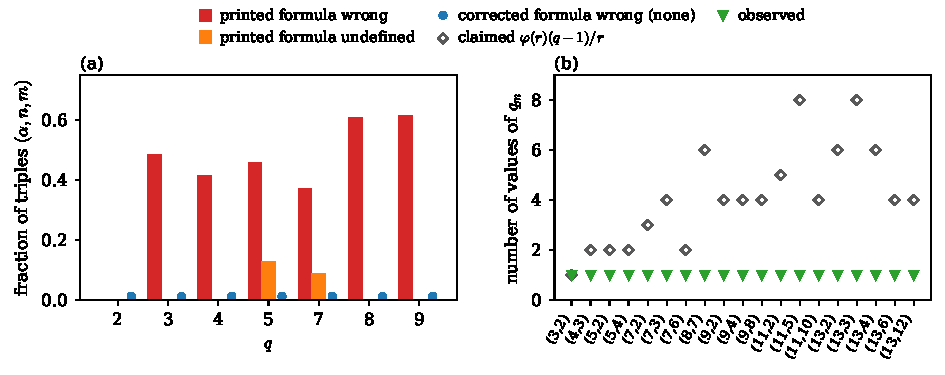
\includegraphics[width=\textwidth]{figures/fig_kapetanakis_jnt2017_1.pdf}
\caption{(a) Fraction of the tested triples $(\alpha,n,m)$ over $\Fq$ for which the coefficient formula of
Theorem~2.8 of \cite{K}, as printed, gives a wrong value or is undefined; formula \eqref{eq:gamma} is correct
in all of them. (b) Number of values of $q_m$ on $\I^A_{n'}$ when $\mu=0$, for pairs $(q,r)$ with $n'=r$,
$m=r-1$, $x_0=-1$: claimed in Theorem~3.4(2) of \cite{K}, and observed.}\label{fig:one}
\end{figure}

\begin{figure}[t]
\centering
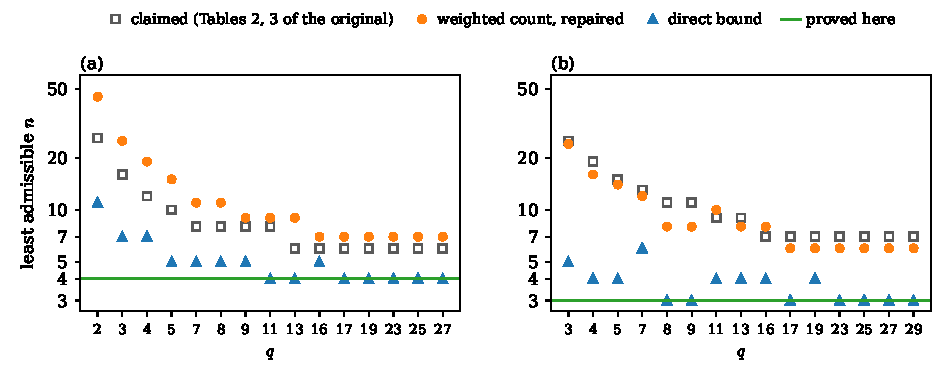
\includegraphics[width=\textwidth]{figures/fig_kapetanakis_jnt2017_2.pdf}
\caption{Least $n_0$ such that the stated condition holds for all $n\ge n_0$ and all admissible $\mu$, by $q$.
(a) One eigenvalue, $2\le\mu\le n/2$: Table~2 of \cite{K}; \eqref{eq:S2}; \eqref{eq:D2}; Theorem~A(4). (b) Two
eigenvalues, $1\le\mu<n/2$, with $W(r)=W(q-1)$: Table~3 of \cite{K}; \eqref{eq:S3}; \eqref{eq:D3};
Theorem~B(3).}\label{fig:two}
\end{figure}

\section{Computations}\label{sec:num}

All statements were tested independently of their proofs.

\emph{Formulas.} \eqref{eq:gamma} was compared with the expansion of $P(X^p-\alpha^{p-1}X)$ for random $P$ in
$1307$ triples $(\alpha,n,m)$, $q\le9$, and the formula $q_m=\sum\delta_ip_{n-i}$, together with the invariance
of $Q$, for $q\le13$: no mismatch. Cohen's criterion in the form $(-1)^np_0\in\fC$ was confirmed by direct
irreducibility tests of $P(X^r)$ in $55$ triples $(q,r,n)$, and Lemmas~\ref{lem:trace} and~\ref{lem:norm} in $39$
pairs $(q,n)$.

\emph{Bounds.} The lower bounds \eqref{eq:D2} and \eqref{eq:D3} were compared with exact counts in $420$ cases
each ($q\le9$, resp.\ $q\le13$; random $c$, $\gamma$, $\delta$; all $\kappa$; all $2\le\mu\le n-1$, resp.\
$1\le\mu\le n-1$): they are never violated, and in the tightest cases the smallest count exceeds a positive
bound by only $4\%$. Proposition~\ref{prop:AB} and the identity $c_k(\psi)=-1$ were checked by computing
$w$ exactly in $234$ cases, and the analogous count behind \eqref{eq:S3} in $162$ cases.

\emph{Finite ranges.} The positivity of \eqref{eq:D2} was evaluated for all prime powers $q<64$ and
$4\le n\le60$, and that of \eqref{eq:D3} for all $3\le q<500$, all $r$ and $4\le n\le60$, and for $n=3$ and all
$q<150000$; the tail inequalities used in Lemmas~\ref{lem:D2pos} and~\ref{lem:D3pos} were checked at the
boundary of these ranges. In the exceptional cases the polynomials were found by a lexicographic search and
tested for irreducibility by the Rabin criterion. The statement A(4) was also confirmed directly on the
polynomials $Q$ in $100$ cases with $q\le5$.

\emph{Code and data availability.} The verification program, its log and its output are archived at
\href{https://doi.org/10.5281/zenodo.24350768}{doi:10.5281/zenodo.24350768} \cite{Repo} and available at
\begin{center}
\url{https://github.com/Ruqing1963/kapetanakis-2017-jnt-audit}
\end{center}

\section{Remarks}\label{sec:rem}

\emph{(1)} Propositions~\ref{prop:D2} and~\ref{prop:D3} are uniform in the linear form: they do not use the
particular values \eqref{eq:gamma}, \eqref{eq:delta}, only $\gamma_\mu\ne0$, resp.\ $\delta_\mu\ne0$. The
exceptional cases were verified in the same uniform sense.

\emph{(2)} Outside the ranges of A(4), A(5), B(3), B(4), that is, for $\mu$ close to $n$, the bounds give
nothing, and for $\mu=n$ the problem changes: for one eigenvalue $m=0$ gives $q_0=p_0$, and for two eigenvalues
with $x_0\ne0$, $m=0$ gives $q_0=P((-x_0)^r)$, which is never $0$. We have not studied these coefficients.

\emph{(3)} Theorems~A and~B depend on \cite{K} only through the cited theorems of Weil, Wan, Agou, Cohen and
Cohen--Pre\v{s}ern. We repeat that our comparison is with the repository text of \cite{K}; statements may have
been changed in print.

\begin{thebibliography}{99}
\bibitem{Ag} S.~Agou, \emph{Factorisation sur un corps fini $\F_{p^n}$ des polyn\^omes compos\'es
$f(X^{p^r}-aX)$ lorsque $f(X)$ est un polyn\^ome irr\'eductible de $\F_{p^n}(X)$}, J.~Number Theory
\textbf{9} (1977), 229--239.
\bibitem{Co} S.~D.~Cohen, \emph{On irreducible polynomials of certain types in finite fields}, Proc.\
Cambridge Philos.\ Soc.\ \textbf{66} (1969), 335--344.
\bibitem{Co2} S.~D.~Cohen, \emph{Primitive polynomials with a prescribed coefficient}, Finite Fields Appl.\
\textbf{12} (2006), 425--491.
\bibitem{CP1} S.~D.~Cohen and M.~Pre\v{s}ern, \emph{Primitive polynomials with prescribed second coefficient},
Glasgow Math.\ J.\ \textbf{48} (2006), 281--307.
\bibitem{CP2} S.~D.~Cohen and M.~Pre\v{s}ern, \emph{The Hansen--Mullen primitivity conjecture: completion of
proof}, in: Number Theory and Polynomials, LMS Lecture Note Ser.\ 352, Cambridge Univ.\ Press, 2008, 89--120.
\bibitem{K} G.~Kapetanakis, \emph{Prescribing coefficients of invariant irreducible polynomials},
J.~Number Theory \textbf{180} (2017), 615--628.
\href{https://doi.org/10.1016/j.jnt.2017.05.003}{doi:10.1016/j.jnt.2017.05.003}.
\bibitem{Repo} R.~Chen, \emph{kapetanakis-2017-jnt-audit: verification program and data}, Zenodo, 2026.
\href{https://doi.org/10.5281/zenodo.24350768}{doi:10.5281/zenodo.24350768}.
\bibitem{Ro} M.~Rosen, \emph{Number Theory in Function Fields}, Grad.\ Texts in Math.\ 210, Springer, 2002.
\bibitem{Wa} D.~Wan, \emph{Generators and irreducible polynomials over finite fields}, Math.\ Comp.\
\textbf{66} (1997), 1195--1212.
\end{thebibliography}
\end{document}
